\chapter{MASSIVE Language}

In this report we illustrates how we designed and implemented the agent oriented language, MASSIVE. During this chapter we demonstrates a working simulation with a use case, and compare the agent oriented language to Object Oriented Code (C\#). Furthermore we discuss the advantages and disadvantages of the MASSIVE language. 

\section{Use Case}
In this use case we demonstrate how to write a mini-game in our language, how to compile it and how to play it. \\
 \\
The first thing one needs to do is to write some MASSIVE code. In \ref{code:MASSIVE} is examples of code, however, there are features of the langauge that are not being used in this example. For a full code referernce please check \ref{} HEJ MED DIG. In the example two teams are created called "Disco" and "Kman", agents are added to them and at the end a simple action pattern is defined, later to be used when running the simulation.

\begin{source}{MASSIVE code example \label{code:MASSIVE}}{}

/* Initializes the game with the properties
Maximum Units = 400 */
Main ( 400 )
{	
	
	// Creates team Disco.
	new team teamDisco("Disco", "#FF6600");
	num totalDiscos = 10;
	for ( num i = 0; i < totalDiscos; i = i + 1)
	{
		num a = 0;
		if ( i < totalDiscos-1 )
		{
			a = 1;
		}
		else
		{
			a = 21-totalDiscos;
		}
		
		new Agent newAgent("Stue", a);
		teamDisco.add(newAgent);
	}
	
	new team teamKman("Kman", "#660000");
	new squad squadNabs("noobs");
	new squad squadRevo("Revolution");
	
	for(num i = 0; i < 4; i = i + 1)
	{
		num a = 0;
		if(i =< 1)
		{
			a = 2;
		}
		if(i >= 2)
		{
			a = 8;
		}
		
		new Agent newAgent("Kman", a);
		teamKman.add(newAgent);
		
		if (i <= 1)
		{
			squadNabs.add(newAgent);
		}
		if (i => 2)
		{
			squadRevo.add(newAgent);
		}
	}
	
	// Moves used in the actionPatterns.
	string moveUp = "unit move up";
	string moveDown = "unit move down";
	string moveLeft = "unit move left";
	string moveRight = "unit move right";
	
	// Creates the action pattern Patrol Low.
	// Patrols the lower part of the game area.
	new actionpattern patrolLow("PatrolLow");
	patrolLow.add(moveUp);
	patrolLow.add("unit move 25,24");
	patrolLow.add(moveUp);
	patrolLow.add("unit move 0,23");
	patrolLow.add(moveDown);
	
}

When compiling this code the compiler warns that there are unused variable (see \ref{fig:compiler}). We will disregard this for the purpose of this use case, however, if there were serious faults in the code the compiler would warn you the same manner and maybe even refuse to compile if the faults were serious enough.

\begin{figure}[h]%
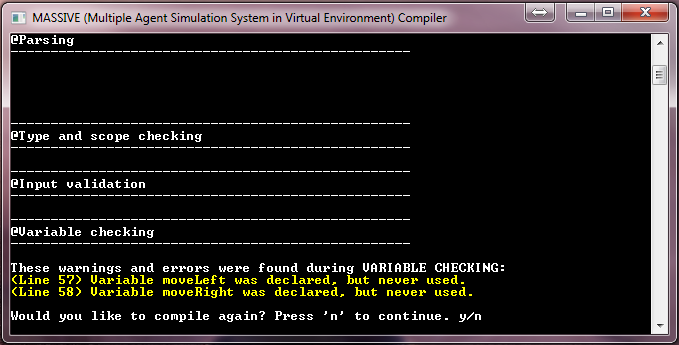
\includegraphics[width=\columnwidth]{image/compiler.png}%
\caption{The MASSIVE compiler warning of unused variables.}%
\label{fig:compiler}%
\end{figure}

The compiler will happily compile the code again if that option is selected, which provides the programmer with an easy way of correcting erroneous code. After a succesfull compilation a file named "MASSIVECode.cs"and "MASSIVECode.exe" will have been created. The only purpose of creating the cs-file is allowing the programmer to have a look at the code our compiler generates. The cs-file will have been compiled into the exe-file wich is run automatically. This exe-file creates the actual data output in XML format, which is then run by the MASSIVE simulator, and the user of the simulator is given a choice of how large the game grid will be (see \ref{fig:game_promt}).

\begin{figure}[h]%
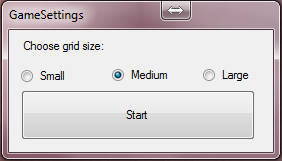
\includegraphics[width=\columnwidth]{images/massive_dialog.png}%
\caption{Choosing the size of the game-grid}%
\label{fig:game_promt}%
\end{figure}

Upon choosing "large", the user will bee presented with the actual simulation (see \ref{fig:runninggame}). Here he will have the oppertunity to instruct the agents to use the action pattern defined in \ref{code:MASSIVE}, as shown in \ref{fig:runninggame}.

\begin{figure}%
\includegraphics[width=\columnwidth]{filename}%
\caption{The simulation running with the input instructing som of the agents to use an actionpattern}%
\label{fig:runninggame}%
\end{figure}

At this point the user is presented with a choice; He can either press "Simulate" to let the simulation run to an end without any interaction, or he can choose to run the game turn-by-turn and control the agents as the game progresses. We see the result of this simulation in \ref{fig:winner}.

\begin{figure}%
\includegraphics[width=\columnwidth]{filename}%
\caption{The result of the use case simulation in MASSIVE}%
\label{fig:winner}%
\end{figure}

\section{OOP}
%Good and bad things about OOP

\section{MASSIVE}
%Good and abd things about MASSIVE
%Why is our MASSIVE better than OOP. 
\section{C\# vs MASSIVE}

\begin{source}{C\# ActionPattern code example}{}                    

\end{source}

\begin{source}{MASSIVE ActionPattern code example}{}                    
	Main(400)
	{
	new ActionPattern ap("Action1");
	ap.add("unit move up");
	ap.add"unit move left");
	ap.add("unit move up");
	}
\end{source}

\begin{source}{C\# Teams code example}{}                    
	
\end{source}

\begin{source}{MASSIVE Teams code example}{}                    
	Main(
\end{source}

\begin{source}{C\# Agent code example}{}                    
	
\end{source}

\begin{source}{MASSIVE Agent code example}{}                    
	Main(400)
	{
	new Agent derp(
	}
\end{source}

\begin{source}{C\# Squad code example}{}                    
	
\end{source}

\begin{source}{MASSIVE Squad code example}{}                    
	
\end{source}

% Her skal vi vise nogle eksempler p� at det er bedre at bruge vores sprog end eksempelvis C\#.
